\section{Progettazione controllori in spazio di stato}
\label{sec:spazioDiStato}	

	In questa sessione si procede alla realizzazione di due tipi di controllori in spazio di stato.
	
	
		
	\subsection{Controllo in feedforward}
	\label{sub:feedforward}
		
		La rappresentazione in spazio di stato permette di fare una retroazione di stato invece che una retroazione dell'uscita, ed è proprio quello che si fa nel \textit{controllo in feedforward}. 
		
		\begin{figure}[H]
			\centering
			\begin{tikzpicture}[auto, node distance=2cm,>=latex']
				\node [input, name=input] {};
				\node [block, right of=input] (N) {$\bar{N}$};
				\node [sum, right of=N] (sum) {};
				\node [block, right of=sum] (xd) {$\dot{x}=Ax+Bu$};
				\node [block, below of=xd] (u) {$u=Kx$};
				\node [input, name=dirama, right of=xd] {};
				\node [block, right of=dirama] (y) {$y=Cx+Du$};
				\node [output, name=output, right of=y] {};
				
				\draw [->] (input) -- node[pos=0.05] {$r(t)$} (N) {};
				\draw [->] (N) -- node[pos=0.4] {$u_{ext}(t)$} node[pos=0.95] {$+$} (sum) {}; 
				\draw [->] (sum) -- node[pos=0.4] {$u(t)$} (xd) {};
				\draw [-] (xd) -- node[pos=0.5] {$x(t)$} (dirama) {};
				\draw [->] (dirama) |- (u) {};
				\draw [->] (u) -| node[pos=0.95] {$-$} (sum) {};
				\draw [->] (dirama) -- (y) {};
				\draw [->] (y) -- node[pos=0.95] {$y(t)$} (output) {};	
			\end{tikzpicture}
			\caption{Schema a blocchi di un controllo in feedforward.}
			\label{fig:feedforward}
		\end{figure}
		
		\noindent Con una retroazione dallo stato, il controllo, e quindi la matrice $K$, viene scelta piazzando i poli in catena chiusa del sistema. Ricordando che un processo può essere scritto in forma di stato come $P(s)=C(sI-A)^{-1}B$, si nota immediatamente che i poli corrispondono agli autovalori  di $sI-A$. Nel sistema complessivo retroazionato, tali autovalori sono di $sI-A+BK$. Il controllo in feedforward, oltre al piazzamento dei poli permette di modificare anche un parametro scalare $\bar{N}$. Per comprendere lo scopo del parametro $\bar{N}$, si pensi di voler riuscire ad inseguire perfettamente un segnale di ingresso costante:
		
		\begin{align*}
			&r(t)=cost \implies y_{DC}=cost \\
			&y_{DC}=P_{CC}(0)r=-C(A-BK)^{-1}Br
		\end{align*} 
		
		\noindent Per sistemi \textit{SISO} $-C(A-BK)^{-1}B$ si riduce ad uno scalare $c$ per cui $y=cr$ e quindi per poter inseguire il riferimento si usa in blocco $\bar{N}$ che cancella il termine $c$. $\bar{N}$ sarà allora scelto nel seguente modo
		
		\begin{equation}
			\bar{N} = \frac{1}{-C(A-BK)^{-1}B}
			\label{eq:Nbarra}
		\end{equation}
		
		\noindent Un possibile problema di questo tipo di controllo è che se non si conoscono perfettamente i valori nominali delle matrici $(A,B,C,D)$, a regime non si riesce ad inseguire perfettamente il riferimento, perchè
		
		\begin{equation}
			y_{DC}=\bar{N}[-C(A-BK)^{-1}B]r_{DC}=\frac{C(A-BK)^{-1}B}{C_{nom}(A_{nom}-B_{nom}K)^{-1}B_{nom}}r_{DC} \ne r_{DC}
		\end{equation}
		
		\noindent Un altro problema è se è presente un disturbo additivo $d(t)$ in ingresso al controllo, infatti risulterebbe
		
		\begin{equation}
			y_{DC}=\alpha r_{DC} + \beta d_{DC}
		\end{equation} 
		
		
		
		
		
		
		
	\subsection{Controllo integrale}
	\label{subsec:ControlloIntegrale}
	
		\begin{figure}[H]
			\centering
			\begin{tikzpicture}[auto, node distance=1.45cm,>=latex']
				\node [input, name=input] {};
				\node [sum, right of=input] (sum1) {};
				\node [block, right of=sum1] (int) {$\int dt$};
				\node [block, right of=int] (kI) {$K_I$};
				\node [sum, right of=kI] (sum2) {};
				\node [output, name=fittizio3, right of=sum2]{};
				\node [sum, right of=fittizio3] (sum3) {};
				\node [output, name=fittizio0, right of=sum3]{};
				\node [block, right of=fittizio0] (sistema){$\dot x=Ax+Bu$};
				\node [input, name=disturbo, above of=sum3] {};
				\node [block, below of=sum3] (K) {$K$};
				\node [output, name=fittizio, below of=K] {};
				\node [output, name=dirama1, right of=sistema] {};
				\node [block, right of=dirama1] (C){$y=Cx$};
				\node [output, name=dirama2, right of=C] {};
				\node [output, name=output, right of=dirama2] {};
			
				\draw [->] (input) -- node[pos=0.05] {$r(t)$} node[pos=0.95] {$+$}(sum1) {};
				\draw [->] (sum1) -- node[pos=0.5] {$e(t)$} (int) {};
				\draw [->] (int) -- node[pos=0.5] {$-x_I$}(kI) {};
				\draw [->] (kI) -- node[pos=0.95] {$+$} (sum2) {};
				\draw [-] (sum2) --  node[pos=0.95] {$u_{ext}(t)$} (fittizio3) {};
				\draw [->] (fittizio3) -- node[pos=0.95] {$+$}(sum3){};
				\draw [->] (disturbo) -| node[pos=0.05] {$d(t)$} node[pos=0.95] {$+$} (sum3){};
				\draw [-] (sum3) -- node[pos=0.5] {$u(t)$}(fittizio0){};
				\draw [->] (fittizio0) -- (sistema){};
				\draw [-] (sistema) -- (dirama1){};
				\draw [->] (dirama1) -- node[pos=0.3] {$x(t)$} (C){};
				\draw [->] (dirama1) |- (K){};
				\draw [->] (K) -| node[pos=0.95] {$-$}(sum2){};
				\draw [-] (C) -- (dirama2){};	
				\draw [->] (dirama2) -- (output) {};
 				\draw [-] (dirama2) |- (fittizio){};
 				\draw [->] (fittizio) -| node[pos=0.95] {$-$} (sum1){}; 
				\draw [->] (C) -- node[pos=0.95] {$y(t)$}(output){};	
			\end{tikzpicture}
			\caption{Schema a blocchi di un controllo integrale con rumore additivo $d(t)$}
			\label{fig:integrale}
		\end{figure}	
	
		\noindent Il controllo integrale è un altro esempio di controllore che sfrutta la retroazione di stato. Prendiamo in considerazione un sistema scritto in forma di stato, dove per semplicità si considera nulla la matrice $D$ \footnote{del tutto lecito visto che il sistema del motore ha appunto $D=0$}
		
		\begin{equation}
			\begin{cases}
				\dot{x}=Ax+Bu \\
				y=Cx
			\end{cases}
			\label{eq:sistemaNoD}
		\end{equation}
	
		\noindent Al sistema viene aggiunto un nuovo stato
		
		\begin{equation}
			\dot{x}_I=e=y-r=Cx-r
			\label{eq:NuovoStato}
		\end{equation}
	
		\noindent ottenendo ancora un sistema dinamico. Si definisce allora un nuovo \textit{stato aumentato} $z \in \mathbb{R}^{n+1}$
		
		\begin{equation}
			z=
			\begin{bmatrix}
				x_I \\
				x
			\end{bmatrix}
			\label{eq:statoAumentato}
		\end{equation}
	
		\noindent e supposto che l'ingresso sia composto da un ingresso di controllo e un disturbo, come in figura \ref{fig:integrale}, $u=u_{ext}+d$ si ottiene
		
		\begin{equation}
			\begin{cases}
				\dot{z}=A_zz+B_zu_z \\
				y_z=C_zz
			\end{cases}
			\label{eq:sistemaIntegrale}
		\end{equation}
		
		\noindent dove $u_z = \begin{bmatrix} u_{ext} \\ d \\ r \end{bmatrix} \in \mathbb{R}^3$ e $y_z=y$. Quindi esplicitando l'equazione \ref{eq:sistemaIntegrale} si ricava
		
		\begin{equation}
			\begin{cases}
				\begin{bmatrix}
					\dot{x}_I \\
					\dot{x}
				\end{bmatrix}
				=
				\underbrace{
				\begin{bmatrix}
					0 & C \\
					0 & A
				\end{bmatrix}
				}_\text{$A_z$}
				\begin{bmatrix}
					x_I \\
					x
				\end{bmatrix}
				+
				\underbrace{
				\begin{bmatrix}
					0 & 0 & -1 \\
					B & B & 0
				\end{bmatrix}
				}_\text{$B_z$}
				\begin{bmatrix}
					u_{ext} \\
					d       \\
					r
				\end{bmatrix} \\
				\\ %
				y=
				\underbrace{
				\begin{bmatrix}
					0 & C
				\end{bmatrix}
				}_\text{$C_z$}
				\begin{bmatrix}
					x_I \\
					x
				\end{bmatrix}
			\end{cases}
			\label{eq:sistemaComplessivo}
		\end{equation}
	
		\noindent Se si definisce $B_z=\begin{bmatrix}B_{ext} & B_{ext} & B_r\end{bmatrix}$ e si sostituisce $u_{ext}=-K_zz$ in \ref{eq:sistemaComplessivo} si ottiene
		
		\begin{equation*}
			\dot{z}=(A_z - B_{ext}K_z)z=
			\begin{bmatrix}
				B_{ext} | B_r
			\end{bmatrix}
			\begin{bmatrix}
				d \\
				r
			\end{bmatrix}
		\end{equation*}
		
		\noindent Quindi, se $A_z-B_{ext}K_z$ è strettamente stabile e gli ingressi sono costanti, $r(t)=r_{DC}$ e $d(t)=d_{DC}$, si rileva che il sistema $z \to z_{cost}$ a $ t \to \infty$.
		\newline Di conseguenza $\dot{z}=\begin{bmatrix}\dot{x}_I \\ \dot{x}\end{bmatrix} \to 0$ che implica $\dot{x}_I \to 0$. Ricordando che $\dot{x}_I=Cx-r=y-r$ si trova che $y \to r$ ottenendo, quindi, un inseguimento perfetto a regime $y \to r \to r_{DC}$.  Se anche $A_z$ e $B_{ext}$ non sono note a priori la matrice $A_z-B_{ext}K_z$ rimane stabile per piccole incertezze, grazie alla \textit{proprietà di continuità} degli autovalori di $A$ rispetto gli elementi di $A$.	
		\newline Rimane ora da verificare che $A_z-B_{ext}K_z$ sia strettamente stabile, questo avviene quando la coppia $(A_z,B_{ext})$ è raggiungibile e quindi con il \textit{criterio PBH} quando $\rank[sI-A_z|B_{ext}]=n+1$. Esplicitando
		
		\begin{equation}
			\begin{bmatrix}
				sI-A_z | B_{ext}
			\end{bmatrix}
			=
			\begin{bmatrix}
			s & -C   & 0 \\
			0 & sI-A & B 
			\end{bmatrix}
		\end{equation}
		
		\noindent si divide la dimostrazione in due parti:
		
		\begin{itemize}
			\item Se $s \ne 0$, $\rank[sI-A_z|B_{ext}]=n+1 \iff \rank[sI-A|B]=n \iff$ la coppia $(A,B)$ è raggiungibile \footnote{questa è una ipotesi necessaria per fare il controllo integrale.}.
			
			\item Se $s=0$, la prima colonna è ininfluente al calcolo e può essere rimossa. Inoltre una eventuale moltiplicazione di righe o colonne per $-1$ così come lo scambio di righe, non cambia il rango, quindi la raggiungibilità per $s=0$ è equivalente a verificare 
			\begin{equation*}
				\rank
				\begin{bmatrix}
					sI-A & -B \\
					C    & 0 
				\end{bmatrix}_{s=0}
				=n+1
			\end{equation*}
			Il rango di questa matrice è $n+1$ se e solo se $s=0$ non è uno zero di $P(s)=C(sI-A)^{-1}B$ \footnote{ulteriore ipotesi necessaria per il controllo integrale.}
		\end{itemize}
		
		\noindent Per quanto riguarda la matrice di retroazione $K$, se le due ipotesi sono verificate, esiste tale che $A_z-B_zK_z$ ha autovalori arbitrari e quindi
		
		\begin{equation}
			u_{ext}(t)=-K_zz(t)=-
			\begin{bmatrix}
				K_I | K
			\end{bmatrix}
			\begin{bmatrix}
				x_I(t) \\
				x(t)
			\end{bmatrix}
			=-K_Ix_I(t)-Kx(t)
		\end{equation}
	
		\noindent Si fa notare che il termine $-K_Ix_I$ può essere scritto come $-K_Ix_I(t)=-K_I\int y(t)-r(t)dt=K_I\int r(t)-y(t)dt$ e rappresentato graficamente in figura \ref{fig:integrale}. 
		\newline  Questo modello risulta più lento rispetto al feed-forward perché l'errore integrale richiede un certo tempo prima che l'effeto sul controllo sia evidente.  
		
		



	\subsection{Piazzamento dei poli in catena chiusa}
	\label{subsec:PoliCatenaChiusa}
	
		Il problema principale di un controllo in spazio di stato, rimane quello di scegliere la posizione dei poli in catena chiusa. Non esistono delle regole matematiche ben precise, ma vi sono degli aspetti da tenere bene in mente quando si usa questo tipo di controllo. Come già accennato, i poli si trovano facilmente come $\det[sI-(A-BK)]$   
		
		\begin{wrapfloat}{figure}{L}{0pt}
			\centering
			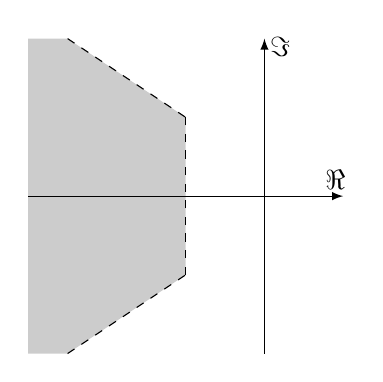
\begin{tikzpicture}[scale=1]
				%\draw[help lines,step=1] (0,0) grid (4,4);
				\draw [-latex] (0,2) -- (4,2);
				\draw [-latex] (3,0) -- (3,4);
				\draw [dashed] (0.5,0) -- (2,1);
				\draw [dashed] (0.5,4) -- (2,3);
				\draw [dashed] (2,1) -- (2,3);
				\fill [fill opacity=0.2] (0,0) -- (0.5,0) -- (2,1) -- (2,3) -- (0.5,4) -- (0,4);			
				
				\node [align=center] at (3.9, 2.2) {$\Re$};
				\node [align=center] at (3.2, 3.9) {$\Im$};	
			\end{tikzpicture}	
			\caption{Regione delle specifiche per sistema del secondo ordine.}
			\label{fig:regioneSpecifiche}			
		\end{wrapfloat}
		
		\noindent e se la coppia $(A,B)$ è raggiungibile esiste sicuramente una matrice $K$ che può posizionare gli autovalori $(A-BK)$ nella posizione desiderata. Utilizzando una approssimazione di un sistema del secondo ordine\footnote{Consultare le note delle lezioni di \textit{Laboratorio di controlli} per una spiegazione accurata \url{http://www.dei.unipd.it/~schenato/didattica/LabControlli1/LC1_Lezione10.pdf}} si ottiene una regione nel piano complesso dove è possibile piazzare i poli come in figura \ref{fig:regioneSpecifiche}. Detto questo, per garantire delle buone prestazioni bisogna solitamente seguire almeno queste tre regole:
		
		\begin{itemize}
			\item Spostare i poli in catena chiusa non troppo negativi, cioè cercare di piazzarli appena dentro la regione che soddisfa le specifiche; questo perché per piazzarli molto negativi, bisogna far crescere il valore della matrice $K$, ciò porta a una amplificazione degli errori di misura.
			
			\item Spostare di poco i poli che sono vicini agli zeri; questo perché se si pensa al \textit{luogo delle radici}, un polo vicino a uno zero avranno un ramo molto piccolo e quindi resterà in un intorno del polo.
			
			\item  Non spostare poli già molto negativi; semplicemente perché non si avrebbe alcun miglioramento pratico e anzi, si andrebbe ad aumentare ancora la matrice $K$.

		\end{itemize}
		
